% version 2.00, date 30/11/16, auteur Julie Pain

\newpage

\section*{}

\section{Diagramme de classes}

Le formalisme utilisé dans ce document pour le diagramme de classe est UML.

%% Inclure le  diagramme de classe
\begin{landscape}
\begin{figure}
	\centering
	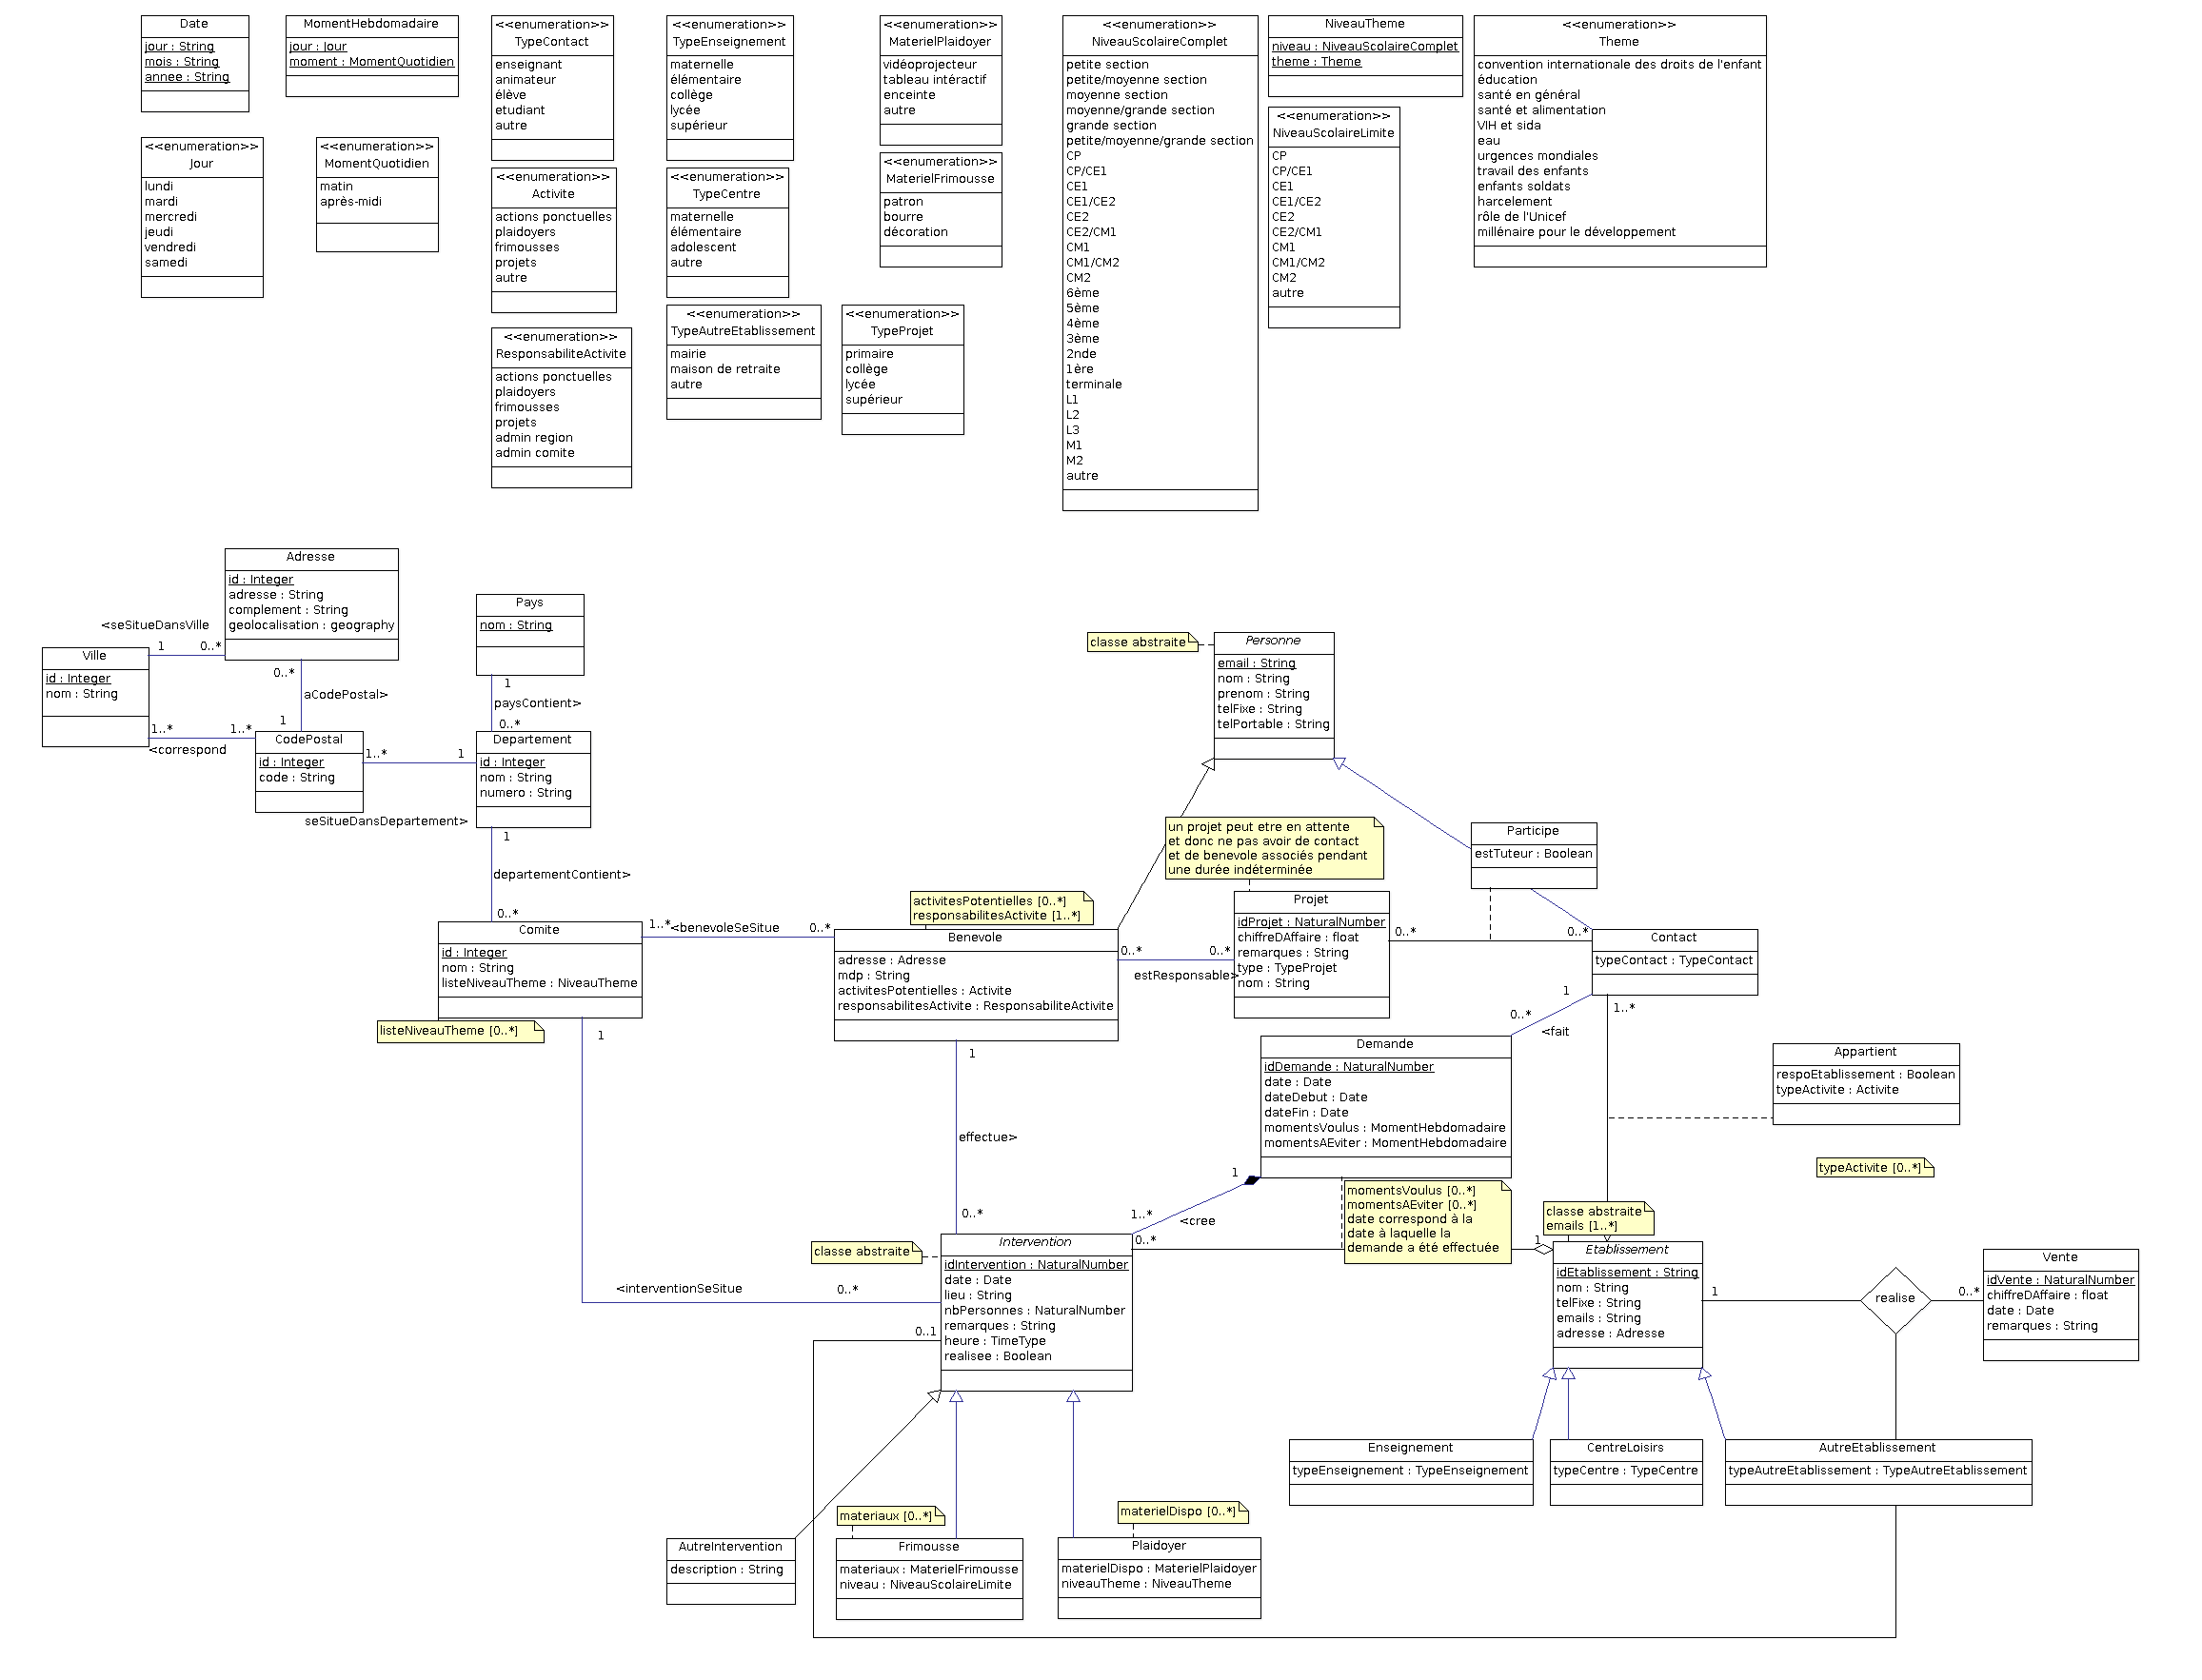
\includegraphics[scale=0.3]{images/diagrammeDeClasses.png}
	\caption{\label{modele}Diagramme de classes}
\end{figure}
\end{landscape}

\section{Description du Diagramme de classes}

Le diagramme de classes réalisé est composé de plusieurs types, de plusieurs classes et de plusieurs associations. \\ 

\subsection{Les types}

\subsubsection*{Geography}

Le type Geography est un type de données respectant la norme de l'OGC (Open Geospatial Consortium) et qui définit la géolocalisation.


\subsubsection*{Date}

La classe Date définit un type qui est une date.\\
Cette classe a plusieurs attributs : 
\begin{itemize}
\item un jour;
\item un mois;
\item une année.
\end{itemize}

\subsubsection*{Jour}

Le type Jour est une énumération qui définit les différents jours possibles pour une intervention.

\subsubsection*{MomentHebdomadaire}

La classe MomentHebdomadaire définit un type qui est la combinaison d'un jour et d'un moment quotidien.\\
Cette classe a plusieurs attributs :
\begin{itemize}
\item un jour qui appartient à l'énumération Jour;
\item un moment qui appartient à l'énumération MomentQuotidien.
\end{itemize}

\subsubsection*{MomentQuotidien}

Le type MomentQuotidien est une énumération qui définit les différents moments possibles dans une journée, donc matin ou après-midi.

\subsubsection*{TypeContact}

Le type TypeContact est une énumération qui définit les différents contacts possibles.

\subsubsection*{Activite}

Le type Activite est une énumération qui définit les différentes activités que peuvent réaliser les bénévoles. Il représente également l'Activité dont un Contact travaillant dans un Etablissement peut être responsable.

\subsubsection*{ResponsabiliteActivite}

Le type ResponsabiliteActivite est une énumération qui définit les différentes activités dont un bénévole peut être responsable, mais également si un bénébole est un administrateur d'un comité et/ou d'une région.

\subsubsection*{TypeProjet}

Le type TypeProjet est une énumération qui définit les différents niveaux pour les projets.

\subsubsection*{TypeEnseignement}

Le type TypeEnseignement est une énumération qui définit les différents niveaux pour les enseignements.

\subsubsection*{TypeCentre}

Le type TypeCentre est une énumération qui définit les différents niveaux pour les centres de loisirs.

\subsubsection*{TypeAutreEtablissement}

Le type TypeAutreEtablissement est une énumération qui définit la nature des établissements qui ne sont pas des enseignements ou des centres de loisirs, par exemple une mairie ou une maison de retraite.

\subsubsection*{MaterielPlaidoyer}

Le type MaterielPlaidoyer est une énumération qui définit les différents types de matériel possibles pour les interventions plaidoyers.

\subsubsection*{MaterielFrimousse}

Le type MaterielFrimousse est une énumération qui définit les différents matériaux possibles pour les interventions frimousses.

\subsubsection*{NiveauScolaireComplet}

Le type NiveauScolaireComplet est une énumération qui définit tous les niveaux possibles pour les interventions plaidoyer. Ce type comporte aussi des combinaisons des niveaux comme par exemple "CP/CE1" ou "CM1/CM2". La valeur "autre" est utilisée pour des cas particuliers (niveau CLIS, CM2/6eme par exemple).

\subsubsection*{NiveauScolaireLimite}

Le type NiveauScolaireLimite est une énumération qui définit tous les niveaux possibles pour les interventions frimousse en se limitant à l'école primaire. Ce type comporte aussi des combinaisons des niveaux comme par exemple "CP/CE1" ou "CM1/CM2". La valeur "autre" est utilisée pour des cas particuliers (niveau CLIS, CM2/6eme par exemple).

\subsubsection*{Theme}

Le type Theme est une énumération qui définit les différents thèmes possibles pour les plaidoyers. Ce type est global pour l'ensemble des interventions quelle que soit la région.  

\subsubsection*{NiveauTheme}

La classe NiveauTheme définit un type qui est la combinaison d'un thème et d'un niveau. En effet, un thème pour un plaidoyer n'est pas forcément présenté à tout type de niveau, cette classe permet donc de faire les liaisons entre les thèmes et les niveaux associés à ces thèmes.\\
Cette classe a plusieurs attributs : 
\begin{itemize}
\item un niveau qui appartient à l'énumération NiveauScolaireComplet;
\item un thème qui appartient à l'énumération Theme.
\end{itemize}


\subsection{Les classes}

\subsubsection*{Personne}

La classe Personne est la classe mère des classes Benevole et Contact. C'est une généralisation, c'est à dire que la classe Personne est une classe abstraite et donc une Personne est soit un contact, soit un bénévole. \\
Cette classe a plusieurs attributs : 
\begin{itemize}
\item un email;
\item un nom;
\item un prénom;
\item un numéro de téléphone fixe;
\item un numéro de téléphone portable.
\end{itemize}

\subsubsection*{Benevole}

La classe Benevole est une classe fille de la classe Personne. Cette classe décrit les bénévoles de l'UNICEF qui réaliseront des interventions mais aussi ceux qui géreront des activités, des comités ou des régions.\\
Cette classe a plusieurs attributs : 
\begin{itemize}
\item une adresse correspondant à la rue, au code postal, à la ville, au complément si besoin et à une géolocalisation;
\item un mot de passe;
\item aucune, une ou plusieurs activités potentielles (action ponctuelle, plaidoyer, frimousse, projet ou autre);
\item aucune, une ou plusieurs responsabilités d'activité (action ponctuelle, plaidoyer, frimousse, projet, admin region ou admin comite). 
\end{itemize}


\subsubsection*{Contact}

La classe Contact est une classe fille de la classe Personne. Cette classe décrit les personnes étant reliées à un établissement comme le personnel y travaillant ou encore les élèves ou étudiants participant à des projets. \\
Cette classe a un attribut : 
\begin{itemize}
\item un type de contact qui permet de déterminer si un contact est un enseignant, un animateur, un élève, un étudiant ou autre.
\end{itemize} 

\subsubsection*{Etablissement}

La classe Etablissement est la classe mère des classes Enseignement, CentreLoisirs et AutreEtablissement. C'est une généralisation, c'est à dire qu'un établissement ne peut être qu'un enseignement, un centre de loisirs ou un autre établissement (pour les mairies par exemple).\\
Cette classe a plusieurs attributs : 
\begin{itemize}
\item un identifiant;
\item un nom;
\item un numéro de téléphone fixe;
\item une ou plusieurs adresses e-mail;
\item une adresse correspondant à la rue, au code postal, à la ville, au complément si besoin et à une géolocalisation.
\end{itemize}

\subsubsection*{Enseignement}
La classe Enseignement est une classe fille de la classe Etablissement. Cette classe décrit les établissements qui relèvent de l'Education Nationale. \\
Cette classe a un attribut : 
\begin{itemize}
\item un type d'enseignement qui permet de déterminer si l'enseignement est une école maternelle, une école élémentaire, un collège, un lycée ou un établissement supérieur. 
\end{itemize} 


\subsubsection*{CentreLoisirs}
La classe CentreLoisirs est une classe fille de la classe Etablissement. Cette classe décrit les établissements ayant un rapport avec les loisirs. \\
Cette classe a un attribut : 
\begin{itemize}
\item un type de centre de loisirs qui permet de déterminer si un centre de loisirs prend en charge des enfants d'école maternelle, d'école élémentaire, des adolescents ou autre.
\end{itemize}  

\subsubsection*{AutreEtablissement}
La classe AutreEtablissement est une classe fille de la classe Etablissement. Cette classe décrit les établissements n'étant ni un enseignement, ni un centre de loisirs. \\
Cette classe a un attribut : 
\begin{itemize}
\item un type qui permet de déterminer si la structure est une mairie, une maison de retraite, ou un autre établissement.
\end{itemize}  

\subsubsection*{Intervention}
La classe Intervention est la classe mère des classes Plaidoyer, Frimousse et AutreIntervention. Cette classe décrit une intervention que peut demander un contact. \\
Cette classe a plusieurs attributs :
\begin{itemize}
\item un identifiant;
\item une date précise déterminée par les bénévoles lors de l'affectation des bénévoles aux interventions;
\item un lieu dans l'établissement, c'est à dire la salle où aura lieu l'intervention;
\item le nombre de personnes concernées par cette intervention (exemple : le nombre d'élèves d'une classe);
\item un champ remarques permettant au contact de saisir des remarques spécifiques à cette intervention;
\item une heure indiquant l'heure à laquelle l'intervention aura lieu;
\item un attribut "realisee" permettant de savoir si une intervention a été réalisée ou non.
\end{itemize}

\subsubsection*{Plaidoyer}
La classe Plaidoyer est une classe fille de la classe Intervention. \\
Cette classe a plusieurs attributs : 
\begin{itemize}
\item le matériel disponible pour l'intervention (présence ou non d'un vidéoprojecteur, d'un tableau interactif, d'enceintes ou autre);
\item un niveauTheme qui indique à la fois le thème de l'intervention et le niveau de la classe dans laquelle va se dérouler l'intervention, par exemple, pour une école primaire, la classe peut être CE1 mais aussi CE1/CE2.
\end{itemize}

\subsubsection*{Frimousse}
La classe Frimousse est une classe fille de la classe Intervention. Une activité frimousse est réalisée avec des enfants d'école élémentaire. \\
Cette classe a plusieurs attributs :
\begin{itemize}
\item les matériaux nécessaires à la réalisation de l'activité (patron, bourre, décoration);
\item un niveau qui correspond à la classe dans laquelle va se dérouler l'intervention (CP, CE1, etc).
\end{itemize}

\subsubsection*{AutreIntervention}
La classe AutreIntervention est une classe fille de la classe Intervention. Une AutreIntervention peut être réalisée dans un dans un établissement et n'est ni un plaidoyer ni une activité frimousse.  \\
Cette classe possède un attribut :
\begin{itemize}
\item une description permettant de décrire cette intervention, en quoi elle consiste et son public par exemple.
\end{itemize}

\subsubsection*{Projet}
La classe Projet représente les projets réalisés par des étudiants ou des élèves.\\
Cette classe a plusieurs attributs : 
\begin{itemize}
\item un identifiant;
\item le chiffre d'affaire réalisé par ce projet;
\item un champs remarques permettant au(x) bénévole(s) de saisir d'autres informations importantes sur le projet;
\item le type de projet permet de savoir si le projet est réalisé par des étudiants, des lycéens, des élèves d'école primaire ou de collège;
\item le nom du projet.
\end{itemize}

\subsubsection*{Vente}
La classe Vente représente les actions ponctuelles réalisées par les établissements.\\ 
Cette classe a plusieurs attributs : 
\begin{itemize}
\item un identifiant; 
\item le chiffre d'affaire réalisé par cette vente;
\item la date de la vente;
\item un champ remarques permettant aux bénévoles d'ajouter des informations importantes. 
\end{itemize}

\subsubsection*{Demande}

La classe Demande représente les demandes d'intervention effectuées par les contacts pour un Etablissement.\\
Cette classe a plusieurs attributs :
\begin{itemize}
\item un identifiant;
\item une date correspondant au moment où la demande a été faite;
\item une date de début correspondant à la date à partir de laquelle l'intervention peut se faire; 
\item une date de fin correspondant à la date butoire pour réaliser l'intervention;
\item les moments voulus pour une semaine type (sera donc valable pour toutes les semaines où le contact est disponible);
\item les moments à éviter pour une semaine type.
\end{itemize}

\subsubsection*{Comite}

La classe Comite représente les comités de bénévoles, il y a en général un comité par département. Il peut arriver qu'un département ne possède pas de comité.\\
Cette classe a plusieurs attributs :
\begin{itemize}
\item un identifiant unique;
\item le nom du comité;
\item la liste des thèmes du comité avec les niveaux associés à chaque thème. Un comité ne présente pas forcément les mêmes thèmes qu'un autre comité et, pour un même thème, les niveaux associés ne sont pas obligatoirement les mêmes en fonction des comités. 
\end{itemize}


\subsubsection*{Departement}

La classe Departement représente les départements de France.\\
Cette classe a plusieurs attributs :
\begin{itemize}
\item un identifiant unique;
\item le nom du département;
\item le numéro du département.
\end{itemize}

\subsubsection*{CodePostal}

La classe CodePostal représente les codes postaux de France.\\
Cette classe a plusieurs attributs : 
\begin{itemize}
\item un identifiant unique;
\item un code correspondant au code postal.
\end{itemize}

\subsubsection*{Ville}

La classe Ville représente les villes de France. \\
Cette classe a plusieurs attributs :
\begin{itemize}
\item un identifiant unique; 
\item le nom de la ville.
\end{itemize}

\subsubsection*{Adresse}

La classe Adresse définit un type qui est l'adresse d'un bénévole ou d'un établissement.\\
Cette classe a plusieurs attributs : 
\begin{itemize}
\item un identifiant unique;
\item une adresse correspondant au numéro de rue et à la rue par exemple;
\item un complément si besoin;
\item la géolocalisation associée à cette adresse.
\end{itemize}


\subsubsection*{Pays}

La classe Pays représente la France.\\
Cette classe a un attribut :
\begin{itemize}
\item le nom du pays (donc "France").
\end{itemize}


\subsection{Les associations}

\subsubsection*{estResponsable}
L'association \textit{estResponsable} relie un Benevole et un Projet. Un bénévole est responsable d'aucun, un ou plusieurs projets et un projet est sous la responsabilité d'aucun (si le projet est en attente), un ou plusieurs bénévoles.

\subsubsection*{Participe}
L'association \textit{Participe} relie un Contact et un Projet. Un contact participe à aucun, un ou plusieurs projets et un projet a pour participant aucun (si le projet est en attente), un ou plusieurs contacts.\\
Cette association a un attribut :
\begin{itemize}
\item un booléen qui indique si le contact est ou non un tuteur du projet (un professeur tuteur des élèves réalisant le projet par exemple). 
\end{itemize}

\subsubsection*{realise}

L'association \textit{realise} est une association ternaire qui relie une Vente, un Etablissement et une Intervention. Un établissement réalise aucune, une ou plusieurs ventes. Une vente est réalisée par un et un seul établissement. La vente a été réalisée suite à aucune ou une intervention.

\subsubsection*{fait}

L'association \textit{fait} relie un Contact et une Demande. Un contact fait aucune, une ou plusieurs demandes, une demande est faite par un et un seul contact.

\subsubsection*{cree}

L'association \textit{cree} relie une Demande et une Intervention. Une demande crée une ou plusieurs interventions, une intervention est créée par une et une seule demande.

\subsubsection*{effectue} 

L'association \textit{effectue} relie un Benevole et une Intervention. Un bénévole effectue aucune, une ou plusieurs interventions. Une intervention est effectuée par un et un seul bénévole. 

\subsubsection*{Appartient}

L'association \textit{Appartient} relie un Contact et un Etablissement. Un contact appartient à aucun, un ou plusieurs établissements. Un établissement a un ou plusieurs contacts.\\
Cette association a plusieurs attributs :
\begin{itemize}
\item un booléen qui indique si le contact est ou non le responsable de l'établissement; 
\item un type qui indique quelles sont les responsabilités du contact par rapport aux activités.
\end{itemize}


\subsubsection*{benevoleSeSitue}

L'association \textit{benevoleSeSitue} relie un Benevole et un Comite. Un bénévole se situe dans un ou plusieurs comités. Un comité a aucun, un ou plusieurs bénévoles.

\subsubsection*{interventionSeSitue}

L'association \textit{interventionSeSitue} relie une Intervention et un Comite. Une intervention se situe dans un et un seul comité. Un comité a aucune, une ou plusieurs interventions.

\subsubsection*{departementContient}

L'association \textit{departementContient} relie un Departement et un Comite. Un département contient aucun, un ou plusieurs comités. Un comité est dans un et un seul département.

\subsubsection*{paysContient}

L'association \textit{paysContient} relie un Pays et un Departement. Un pays contient aucun, un ou plusieurs départements. Un département est dans un et un seul pays.


\subsubsection*{seSitueDansDepartement}

L'association \textit{seSitueDansDepartement} relie un Departement et un CodePostal. Un codePostal se situe dans un et un seul département. Un département possède un à plusieurs codes postaux. 

\subsubsection*{correspond}

L'association \textit{correspond} relie un CodePostal et une Ville. Un code postal correspond à une ou plusieurs villes. Une ville correspond à un ou plusieurs code postaux.

\subsubsection*{seSitueDansVille}

L'association \textit{seSitueDansVille} relie une Ville et une Adresse. Une adresse se situe dans une et une seule ville. Une ville contient aucune ou plusieurs adresses.

\subsubsection*{aCodePostal}

L'association \textit{aCodePostal} relie une Adresse et un CodePostal. Une adresse a un et un seul code postal. Un code postal peut correspondre à aucune ou plusieurs adresses. 

\section{Contraintes d'intégrité}

Les contraintes d'intégrité portent sur l'intra-classe et l'inter-classe.

\subsection{Les contraintes d'intégrité intra-classe}
Dans cette partie, nous allons décrire les différentes contraintes d'intégrité de chaque classe et classe-association.

\subsubsection{Classe} 
 
\subsubsection*{Personne}
Contraintes de domaine et de nullité des attributs :
\begin{itemize}
	\item \textbf{email :} chaîne de caractère de longueur de 100 caractères au maximum, la syntaxe de l'e-mail doit être la suivante : user@host.domain\\
	user : contient des chiffres/lettres ainsi que les symboles "\_", "-", "." \\
	host : contient des chiffres/lettres \\
	domain : chaine de caractère composée de 2 lettres au minimum et 3 lettres au maximum. \\
	attribut non nul;  
 	\item \textbf{nom :} chaîne de caractère de longueur de 100 caractères au maximum, attribut non nul;
	\item \textbf{prénom :} chaîne de caractère de longueur de 100 caractères au maximum, attribut peut être nul;
	\item \textbf{telFixe :} chaîne de caractère composée de 10 chiffres commençant par "0", attribut peut être nul;
	\item \textbf{telPortable :} chaîne de caractère composée de 10 chiffres commençant par "0", attribut peut être nul.\\
\end{itemize}  

Clés : 

L'\textbf{email} est unique.\\

\subsubsection*{Benevole}
Contraintes de domaine et de nullité des attributs :
\begin{itemize}
 	\item \textbf{adresse :} variable de type \textbf{Adresse}, attribut non nul;
	\item \textbf{mdp :} chaîne de caractère de longueur de 50 caractères au maximum, de 8 caractères au minimum, attribut non nul;  
	\item \textbf{activitesPotentielles :} constante de type \textbf{Activite}, attribut multivalué, attribut  peut être nul;
	\item \textbf{responsabilitesActivite :} constante de type \textbf{ResponsabiliteActivite}, attribut multivalué, peut être nul.\\
\end{itemize}  
 
\subsubsection*{Contact}
Contraintes de domaine et de nullité des attributs :
 \begin{itemize}
 \item \textbf{type :} constante de type \textbf{TypeContact},attribut non nul.\\
 \end{itemize}

\subsubsection*{Etablissement}
Contraintes de domaine et de nullité des attributs :
\begin{itemize}
 	\item \textbf{idEtablissement :} chaîne de caractère de longueur de 100 caractères au maximum, attribut non nul. Cet attribut doit correspondre à l'UAI si cet établissement est une instance d'Enseignement. L'UAI (Unité Administrative Immatriculée) qui est une combinaison de chiffres et de lettres unique pour chaque enseignement;
	\item \textbf{nom :} chaîne de caractère de longueur de 100 caractères au maximum, attribut peut être nul;
	\item \textbf{telFixe :} chaîne de caractère composée de 10 chiffres commençant par "0", attribut peut être nul;
	\item \textbf{emails :} chaîne de caractère de longueur de 100 caractères au maximum, la syntaxe de l'e-mail doit être la suivante : user@host.domain\\
	user : contient des chiffres/lettres ainsi que les symboles "\_", "-", "." \\
	host : contient des chiffres/lettres \\
	domain : chaîne de caractère composée de 2 ou 3 lettres. \\
	attribut multivalué, non nul; 
	\item \textbf{adresse :} variable de type \textbf{Adresse}, attribut non nul.\\
\end{itemize}  

Clés : 
\begin{itemize}
\item clé structurelle : \textbf{idEtablissement} est unique;
\item clé sémantique : \textbf{adresse} et \textbf{type} est une autre clé candidate. \\ 
\end{itemize}

\subsubsection*{Enseignement}
Contraintes de domaine et de nullité des attributs :
\begin{itemize}
	\item \textbf{typeEnseignement :} constante de type \textbf{TypeEnseignement}, attribut non nul.\\
\end{itemize}

\subsubsection*{CentreLoisirs}
Contraintes de domaine et de nullité des attributs :
\begin{itemize}
	\item \textbf{typeCentre :} constante de type \textbf{TypeCentre}, attribut non nul.\\
\end{itemize}

\subsubsection*{AutreEtablissement}
Contraintes de domaine et de nullité des attributs :
\begin{itemize}
	\item \textbf{typeAutreEtablissement :} constante de type \textbf{TypeAutreEtablissement}, attribut non nul.\\
\end{itemize}

\subsubsection*{Intervention} 
Contraintes de domaine et de nullité des attributs :
\begin{itemize}
 	\item \textbf{idIntervention :} entier positif ou nul, attribut non nul;
	\item \textbf{date :} variable de type \textbf{Date}, attribut peut être nul;
	\item \textbf{lieu :} chaîne de caractère composée de chiffres et de lettres, attribut peut être nul;
	\item \textbf{nbPersonnes :} entier positif non nul, attribut non nul;  
	\item \textbf{remarques :} chaîne de caractères de longueur de 1000 caractères au maximum, peut être nul;
	\item \textbf{heure :} constante de type \textbf{Time}, attribut peut être nul;
	\item \textbf{realisee :} booléen, attribut non nul. \\
\end{itemize}  

Clés : 
\begin{itemize}
\item clé structurelle : \textbf{idIntervention} est unique;
\item clé sémantique : \textbf{heure} (Intervention), \textbf{date} (Intervention), \textbf{nom} (Benevole), \textbf{prenom} (Benevole), \textbf{type} (Etablissement) et \textbf{adresse} (Etablissement) est une autre clé candidate. \\ 
\end{itemize}

\subsubsection*{Plaidoyer}
Contraintes de domaine et de nullité des attributs :
\begin{itemize}
	\item \textbf{materielDispo :} constante de type \textbf{MatérielPlaidoyer}, attribut multivalué peut être nul; 
	\item \textbf{niveauTheme :} constante de type \textbf{niveauTheme}, attribut non nul.\\
\end{itemize}

\subsubsection*{Frimousse}
Contraintes de domaine et de nullité des attributs :
\begin{itemize}
	\item \textbf{materiaux :} constante de type \textbf{MaterielFrimousse}, attribut multivalué peut être nul;
	\item \textbf{niveau :} constante de type \textbf{NiveauScolaireLimite}, attribut non nul.\\
\end{itemize}

\subsubsection*{AutreIntervention}
Contraintes de domaine et de nullité des attributs :
\begin{itemize}
\item \textbf{description :} chaîne de caractères de longueur de 5000 caractères au maximum, attribut non nul.\\
\end{itemize}

\subsubsection*{Projet}
Contraintes de domaine et de nullité des attributs :
\begin{itemize}
 	\item \textbf{idProjet :} entier positif ou nul, attribut non nul;
	\item \textbf{chiffreDAffaire :} réel positif, attribut non nul;
	\item \textbf{remarques :} chaîne de caractère composée de longueur de 1000 caractères au maximum, attribut peut être nul;
	\item \textbf{type :} constante de type \textbf{TypeProjet}, attribut non nul;
	\item \textbf{nom :} chaîne de caractère composée de longueur de 1000 caractères au maximum, attribut non nul.\\  
\end{itemize} 

Clés : 
\begin{itemize}
\item clé structurelle : \textbf{idProjet} est unique;
\item clé sémantique : \textbf{nom} (Projet), \textbf{nom} (Benevole), \textbf{prenom} (Benevole), \textbf{nom} (Contact) et \textbf{prenom} (Contact) est une autre clé candidate. \\ 
\end{itemize}

\subsubsection*{Vente}
Contraintes de domaine et de nullité des attributs :
\begin{itemize}
 	\item \textbf{idVente :} entier positif ou nul, attribut non nul;
	\item \textbf{chiffreDAffaire :} réel positif, attribut non nul;
	\item \textbf{date :} variable de type \textbf{Date}, attribut non nul;
	\item \textbf{remarques :} chaîne de caractères de longueur de 1000 caractères au maximum, peut être nul. \\  
\end{itemize} 

Clés : 

L'\textbf{idVente} est unique.\\

\subsubsection*{Demande}
Contraintes de domaine et de nullité des attributs :
\begin{itemize}
	\item \textbf{idDemande :} entier positif ou nul, attribut non nul;
	\item \textbf{date :} variable de type \textbf{Date}, attribut non nul;
 	\item \textbf{dateDebut :} constante de type \textbf{Date}, attribut non nul;
 	\item \textbf{dateFin :} constante de type \textbf{Date}, attribut non nul;  
	\item \textbf{momentsVoulus :} constante de type \textbf{MomentHebdomadaire}, attribut multivalué peut être nul;
	\item \textbf{momentsAEviter :} constante de type \textbf{MomentHebdomadaire}, attribut multivalué peut être nul.\\
\end{itemize} 

Clés : 
\begin{itemize}
\item clé structurelle : \textbf{idDemande} est unique;
\item clé sémantique : \textbf{date} (Demande), \textbf{type} (Etablissement), \textbf{adresse} (Etablissement), \textbf{nom} (Contact) et \textbf{prenom} (Contact) est une autre clé candidate. \\ 
\end{itemize}

\subsubsection*{Comite}
Contraintes de domaine et de nullité des attributs :
\begin{itemize}
	\item \textbf{id :} entier positif ou nul, attribut non;
	\item \textbf{nom :} chaîne de caractère de longueur de 100 caractères au maximum, attribut non nul;
	\item \textbf{listeNiveauTheme :} constante de type \textbf{NiveauTheme}, attribut multivalué peut être nul. \\
\end{itemize}

Clés : 
\begin{itemize}
\item clé structurelle : \textbf{idDepartement} est unique;
\item clé sémantique : \textbf{nomDepartement} est une autre clé candidate. \\ 
\end{itemize}

\subsubsection*{Departement}
Contraintes de domaine et de nullité des attributs :
\begin{itemize}
	\item \textbf{id :} entier positif ou nul, attribut non;
	\item \textbf{nom :} chaîne de caractère unique de longueur de 100 caractères au maximum, attribut non nul.\\
\end{itemize}

Clés : 
\begin{itemize}
\item clé structurelle : \textbf{idDepartement} est unique;
\item clé sémantique :  \textbf{nom} est une autre clé candidate. \\ 
\end{itemize}

\subsubsection*{CodePostal}
Contraintes de domaine et de nullité des attributs :
\begin{itemize}
	\item \textbf{id :} entier positif ou nul, attribut non;
	\item \textbf{code :} chaîne de caractère unique de longueur de 5 caractères contenant des chiffres allant de 0 à 9, attribut non nul.\\
\end{itemize}

Clés : 
\begin{itemize}
\item clé structurelle : \textbf{id} est unique;
\item clé sémantique :  \textbf{code} est une autre clé candidate. \\ 
\end{itemize}

\subsubsection*{Ville}
Contraintes de domaine et de nullité des attributs :
\begin{itemize}
	\item \textbf{id :} entier positif ou nul, attribut non;
	\item \textbf{nom :} chaîne de caractère unique de longueur de 100 caractères maximum, attribut non nul.\\
\end{itemize}

Clés : 
\begin{itemize}
\item clé structurelle : \textbf{id} est unique;
\item clé sémantique :  \textbf{nom} est une autre clé candidate. \\ 
\end{itemize}


\subsubsection*{Adresse}
Contraintes de domaine et de nullité des attributs :
\begin{itemize}
	\item \textbf{id :} entier positif ou nul, attribut non;
	\item \textbf{adresse :} chaîne de caractère de longueur de 500 caractères au maximum, attribut non nul;
	\item \textbf{complement : } chaîne de caractère de longueur de 100 caractères au maximum, attribut peut être nul;
	\item \textbf{geolocalisation : } attribut de type geoography, peut être nul.\\
\end{itemize}

Clés : 
\begin{itemize}
\item clé structurelle : \textbf{id} est unique;
\item clé sémantique :  \textbf{geolocalisation} est une autre clé candidate. \\ 
\end{itemize}


\subsubsection*{Pays}
Contraintes de domaine et de nullité des attributs :
\begin{itemize}
	\item \textbf{nom :} chaîne de caractère unique de longueur de 100 caractères au maximum, attribut non nul. \\
\end{itemize}

Clés : 
\begin{itemize}
\item clé structurelle : \textbf{nom} est unique. \\ 
\end{itemize}


\subsubsection*{Date}
Contraintes de domaine et de nullité des attributs :
\begin{itemize}
	\item \textbf{jour :} chaîne de caractère de la forme XX, attribut non nul;
	\item \textbf{mois :} chaîne de caractère de la forme XX, attribut non nul;  
	\item \textbf{annee :} chaîne de caractère de la forme XXXX, attribut non nul. 
\end{itemize}

\subsubsection*{NiveauTheme}
Contraintes de domaine et de nullité des attributs :
\begin{itemize}
	\item \textbf{niveau :} constante de type \textbf{NiveauScolaireComplet}, attribut non nul;
	\item \textbf{theme :} constante de type \textbf{Theme}, attribut non nul.\\
\end{itemize}

Autres contraintes :

C'est le comité qui définira l'association entre les thèmes et les niveaux. Il pourra par exemple définir des contraintes de la forme suivante :

Si le niveau est "petite section", "petite/moyenne section", "moyenne section", "moyenne/grande section", "grande section", ou "petite/moyenne/grande section", le thème associé doit être un des thèmes suivants : "convention internationale des droits de l'enfant", "éducation", "santé et alimentation", "eau" et "harcèlement". \\

%Si le niveau est "CP", "CPCE1", "CE1", "CE1CE2", "CE2", "CE2CM1", "CM1", "CM1CM2" ou "CM2", le thème associé doit être un des thèmes suivants : "conventionInternationaleDesDroitsDeLEnfant", "education", "laSanteEnGeneral", "santeAlimentation", "eau", "travailDesEnfants" et "harcelement".
%
%Si le niveau est "6eme", "5eme", "4eme" ou "3eme", le thème associé doit être un des thèmes suivants : "conventionInternationaleDesDroitsDeLEnfant", "education", "laSanteEnGeneral", "santeAlimentation", "eau", "urgencesMondiales", "travailDesEnfants", "enfantsSoldats" et "harcelement".
%
%Si le niveau est "2nde", "1ere", "terminale", "L1", "L2", "L3", "M1", "M2" ou "autre" le thème associé doit être un des thèmes suivants : "conventionInternationaleDesDroitsDeLEnfant", "education", "laSanteEnGeneral", "santeAlimentation", "vihSida", "eau", "urgencesMondiales", "travailDesEnfants", "enfantsSoldats", "harcelement", "roleDeLUnicef" et "millenairePourLeDeveloppement".\\

\subsubsection{Classe-association}

\subsubsection*{Participe}
Contraintes de domaine et de nullité des attributs :
\begin{itemize}
	\item \textbf{estTuteur :} booléen, attribut non nul.\\
\end{itemize}

\subsubsection*{Appartient}
Contraintes de domaine et de nullité des attributs :
\begin{itemize}
	\item \textbf{respoEtablissement :} booléen, attribut non nul;
	\item \textbf{type :} constante de type \textbf{Activite}, attribut multivalué peut être nul.
\end{itemize}


\subsection{Les contraintes d'intégrités inter-classe}


\subsubsection*{Intervention - Etablissement}
Le \textbf{niveau} d'une intervention frimousse ainsi que le \textbf{niveau} (de NiveauTheme) d'une intervention plaidoyer doit être en correspondance avec le \textbf{type} de l'établissement.  

Si l'établissement est un enseignement, le \textbf{niveau} peut prendre différentes valeurs selon le \textbf{type}:
\begin{itemize}
\item Si le \textbf{type} est "maternelle", le \textbf{niveau} peut être : "petite section", "petite/moyenne section", "moyenne section", "moyenne/grande section", "grande section", "petite/moyenne/grande section" ou "autre";
\item Si le \textbf{type} est "elementaire", le \textbf{niveau} peut être : "CP", "CP/CE1", "CE1", "CE1/CE2", "CE2", "CE2/CM1", "CM1", "CM1/CM2", "CM2" ou "autre";
\item Si le \textbf{type} est "college", le \textbf{niveau} peut être : "6eme", "5eme", "4eme", "3eme" ou "autre";
\item Si le \textbf{type} est "lycee", le \textbf{niveau} peut être : "2nde", "1ere", "terminale" ou "autre";
\item Si le \textbf{type} est "superieur", le \textbf{niveau} peut être : "L1", "L2", "L3", "M1", "M2" ou "autre".
\end{itemize}

Si l'établissement est un centre de loisirs, le \textbf{niveau} peut prendre différentes valeurs selon le \textbf{type}:
\begin{itemize}
\item Si le \textbf{type} est "maternelle", le \textbf{niveau} peut être : "petite section", "petite/moyenne section", "moyenne section", "moyenne/grande section", "grande section", "petite/moyenne/grande section" ou "autre";
\item Si le \textbf{type} est "elementaire", le \textbf{niveau} peut être : "CP", "CP/CE1", "CE1", "CE1/CE2", "CE2", "CE2/CM1", "CM1", "CM1/CM2", "CM2" ou "autre";
\item Si le \textbf{type} est "adolescent", le \textbf{niveau} peut être : "6eme", "5eme", "4eme", "3eme", "2nde", "1ere", "terminale" ou "autre". 
\end{itemize}

\subsubsection*{Intervention - Demande}
Les \textbf{momentsVoulus} et \textbf{momentsAEviter} sont dépendants de l'Intervention demandée. En effet, si l'intervention demandée est un Plaidoyer ou une Frimousse, alors les \textbf{momentsQuotidien} dans \textbf{momentHebdomadaire} peuvent être "matin" ou "après-midi". En revanche, si l'intervention demandée est une AutreIntervention, alors les \textbf{momentsQuotidien} dans \textbf{momentHebdomadaire} peuvent être "matin", "après-midi" ou "soir". 
  

\section{Les dépendances}

Dans cette partie, nous allons déterminer les dépendances fonctionnelles, les dépendances multivaluées,  les dépendances d'inclusion et les dépendances d'exclusion. \\

\subsection{Les dépendances fonctionnelles}

Dans cette sous-partie, nous allons déterminer les dépendances fonctionnelles des classes et des associations.  

\subsubsection*{Personne}
\begin{itemize}
\item[] email $\rightarrow$ nom 
\item[] email $\rightarrow$ prenom 
\item[] email $\rightarrow$ telFixe 
\item[] email $\rightarrow$ telPortable 
\item[] telPortable $\rightarrow$ nom
\item[] telPortable $\rightarrow$ prenom
\item[] telFixe $\rightarrow$ nom
\end{itemize}


\subsubsection*{Contact}
\begin{itemize}
\item[] email $\rightarrow$ type 
\end{itemize}

\subsubsection*{Benevole}
\begin{itemize}
\item[] email $\rightarrow$ adresse 
\item[] email $\rightarrow$ mdp 
\end{itemize}


\subsubsection*{Etablissement}
\begin{itemize}
\item[] idEtablissement $\rightarrow$ nom 
\item[] idEtablissement $\rightarrow$ telFixe
\item[] idEtablissement $\rightarrow$ adresse
\item[] telFixe $\rightarrow$ nom
\item[] adresse $\rightarrow$ nom
\item[] adresse, type $\rightarrow$ nom
\item[] adresse, type $\rightarrow$ telFixe
\end{itemize}

\subsubsection*{CentreLoisirs}
\begin{itemize}
\item[]	idEtablissement $\rightarrow$ type
\end{itemize}

\subsubsection*{Enseignement}
\begin{itemize}
\item[]	idEtablissement $\rightarrow$ type
\end{itemize}

\subsubsection*{Intervention}
\begin{itemize}
\item[]	idIntervention $\rightarrow$ date
\item[]	idIntervention $\rightarrow$ dateDebut
\item[]	idIntervention $\rightarrow$ dateFin
\item[]	idIntervention $\rightarrow$ lieu
\item[]	idIntervention $\rightarrow$ nbPersonnes
\item[]	idIntervention $\rightarrow$ remarques
\item[]	idIntervention $\rightarrow$ heure
\item[] heure (Intervention), date (Intervention), type (Etablissement), adresse (Etablissement), nom (Benevole), prenom (Benevole) $\rightarrow$ lieu (Intervention)
\item[] heure (Intervention), date (Intervention), type (Etablissement), adresse (Etablissement), nom (Benevole), prenom (Benevole) $\rightarrow$ nbPersonnes (Intervention)
\item[] heure (Intervention), date (Intervention), type (Etablissement), adresse (Etablissement), nom (Benevole), prenom (Benevole) $\rightarrow$ remarques (Intervention)
\end{itemize}

\subsubsection*{Plaidoyer}
\begin{itemize}
\item[]	idIntervention $\rightarrow$ niveauTheme
\end{itemize}

\subsubsection*{Frimousse}
\begin{itemize}
\item[] idIntervention $\rightarrow$ niveau
\end{itemize}

\subsubsection*{AutreIntervention}
\begin{itemize}
\item[] idIntervention $\rightarrow$ description
\end{itemize}

\subsubsection*{Projet}
\begin{itemize}
\item[] idProjet $\rightarrow$ chiffreDAffaire
\item[] idProjet $\rightarrow$ remarques
\item[] idProjet $\rightarrow$ nom
\item[] idProjet $\rightarrow$ type
\item[]	nom (Projet), nom (Benevole), prenom (Benevole), nom (Contact), prenom (Contact) $\rightarrow$ chiffreDAffaire (Projet)
\item[]	nom (Projet), nom (Benevole), prenom (Benevole), nom (Contact), prenom (Contact) $\rightarrow$ description (Projet)
\item[]	nom (Projet), nom (Benevole), prenom (Benevole), nom (Contact), prenom (Contact) $\rightarrow$ type (Projet)
\item[]	nom (Projet), nom (Benevole), prenom (Benevole), nom (Contact), prenom (Contact) $\rightarrow$ estTuteur (Participe)
\end{itemize}

\subsubsection*{Vente}
\begin{itemize}
\item[]	idVente $\rightarrow$ chiffreDAffaire
\item[]	idVente $\rightarrow$ date
\item[]	idVente $\rightarrow$ remarques
\end{itemize}

\subsubsection*{Demande}
\begin{itemize}
\item[] idDemande $\rightarrow$ date
\end{itemize}

\subsubsection*{Comite}
\begin{itemize}
\item[] id $\rightarrow$ nomDepartement
\end{itemize}

 
\subsubsection*{réalise}
\begin{itemize}
\item[] adresse (Etablissement), type (Etablissement), date (Vente) $\rightarrow$ chiffreDAffaire (Vente)
\item[] adresse (Etablissement), type (Etablissement), date (Vente) $\rightarrow$ date (Intervention), moment (Intervention)
\end{itemize}

\subsection{Les dépendances multivaluées}

\subsubsection*{Benevole}
\begin{itemize}
\item[] email $\rightarrow > $ activitesPotentielles 
\item[]email $\rightarrow >$ activitesPotentielles 
\end{itemize}


\subsubsection*{Etablissement}
\begin{itemize}
\item[] idEtablissement $\rightarrow >$ emails
\item[] adresse, type $\rightarrow$ emails
\end{itemize}

\subsubsection*{Plaidoyer}
\begin{itemize}
\item[]	idIntervention $\rightarrow >$ materielDispo
\end{itemize}

\subsubsection*{Frimousse}
\begin{itemize}
\item[]	idIntervention $\rightarrow >$ materiaux
\end{itemize}

\subsubsection*{Demande}
\begin{itemize}
\item[] idDemande $\rightarrow$ momentsVoulus
\item[] idDemande $\rightarrow$ momentsAEviter
\item[] nom (Contact), prenom (Contact), adresse (Etablissement), type (Etablissement), date (Demande) $\rightarrow$ momentsAEviter (Demande) 
\item[] nom (Contact), prenom (Contact), adresse (Etablissement), type (Etablissement), date (Demande) $\rightarrow$ momentsVoulus (Demande) 
\end{itemize}

\subsubsection*{Comite}
\begin{itemize}
\item[] idDepartement $\rightarrow >$ listeNiveauTheme
\item[] nomDepartement $\rightarrow >$ listeNiveauTheme
\end{itemize}

\subsection{Les dépendances d'inclusion}

\subsubsection*{Plaidoyer - Comite}
Le \textbf{niveauTheme} de Plaidoyer doit faire parti de \textbf{listeNiveauTheme} de Comite.\\
\indent \indent Plaidoyer[niveauTheme] $ \subseteq $ Comite[listeNiveauTheme]

\subsection{Les dépendances d'exclusion}

\subsubsection*{Demande}
L'intersection entre \textbf{momentsVoulus} et \textbf{momentsAEviter} dans Demande doit être nulle. \\
\indent \indent Demande[momentsVoulus] $ \cap $ Demande[momentsAEviter] = 0
